\chapter{Arkitektur}\label{ch:Arkitektur}

Arkitekturen af programmet bestemmer hvordan systemet skal organiseres, samt hvordan de forskellige komponenter skal kommunikere med hinanden. Ved brug af den agile tilgang, er software design noget som burde være i fokus i starten af projektet, da inkrementel udvikling af arkitekturen ofte kan give vanskeligheder. I den agile tilgang, hvor der laves ændringer tit, og hvor nye komponenter skal kobles sammen med resten af systemet, kan arkitekturen hurtigt blive noget rod. refaktorering af de enkelte komponenter kan være nemt, men refaktorering af selve arkitekturen kan være en dyr process, da der efterhånden skal tilpasses flere og flere komponenter. Dette vil ende ud i en forsinkelse af systemets videreudvikling, som påvirker hvor effektivt man kan implementere nyt senere i processen. Derfor er arkitekturen en proces, som gerne skal fastslåes i starten af et software projekt. \cite{Sommerville}

Til dette har gruppen forudbestemt, hvordan arkitekturen skal se ud inden implementering af systemet. Her har der været fokus på hvilke services der skulle være, samt hvordan de skal kommunikere med hinanden. Der er her udviklet en arkitektur model, domænemodel og en relationel model. De beskriver tilsammen de forskellige projekter i applikationen, samt model- og database design. 

\begin{figure}
    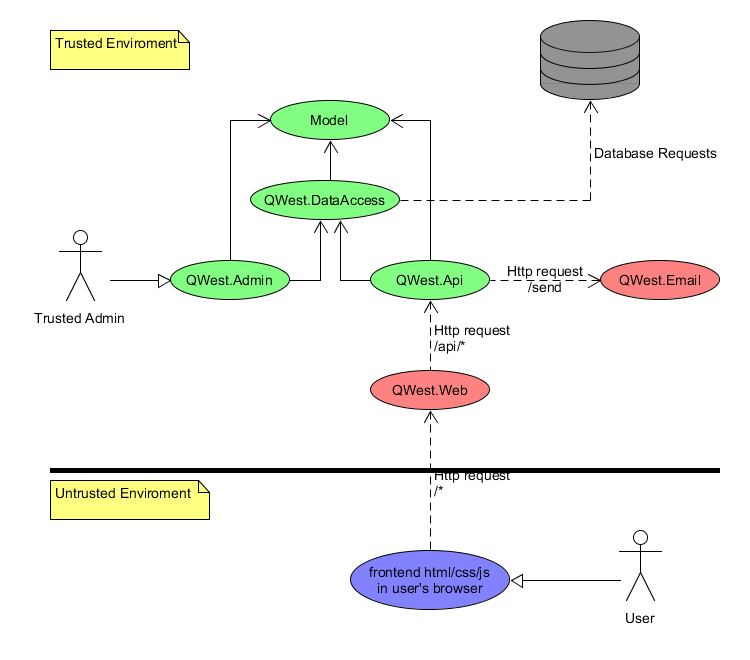
\includegraphics[width=\linewidth]{figures/Architecture.png}
    \caption{Systemets generelle arkitektur}
    \label{fig:Architecture}
\end{figure}

Der er i arkitekturen taget højde for både admin adgang og bruger adgang. Dette kan ses på QWest.Admin og QWest.Api, hvor kun brugeren benytter sig af Web og front-end. Dette skyldes at front-end ikke er et miljø hvor der kan være blind tiltro til brugeren, og der er barriere mellem bruger og databasen, så databasen ikke kan redigeres uden særlig tilladelse. 

\begin{figure}
    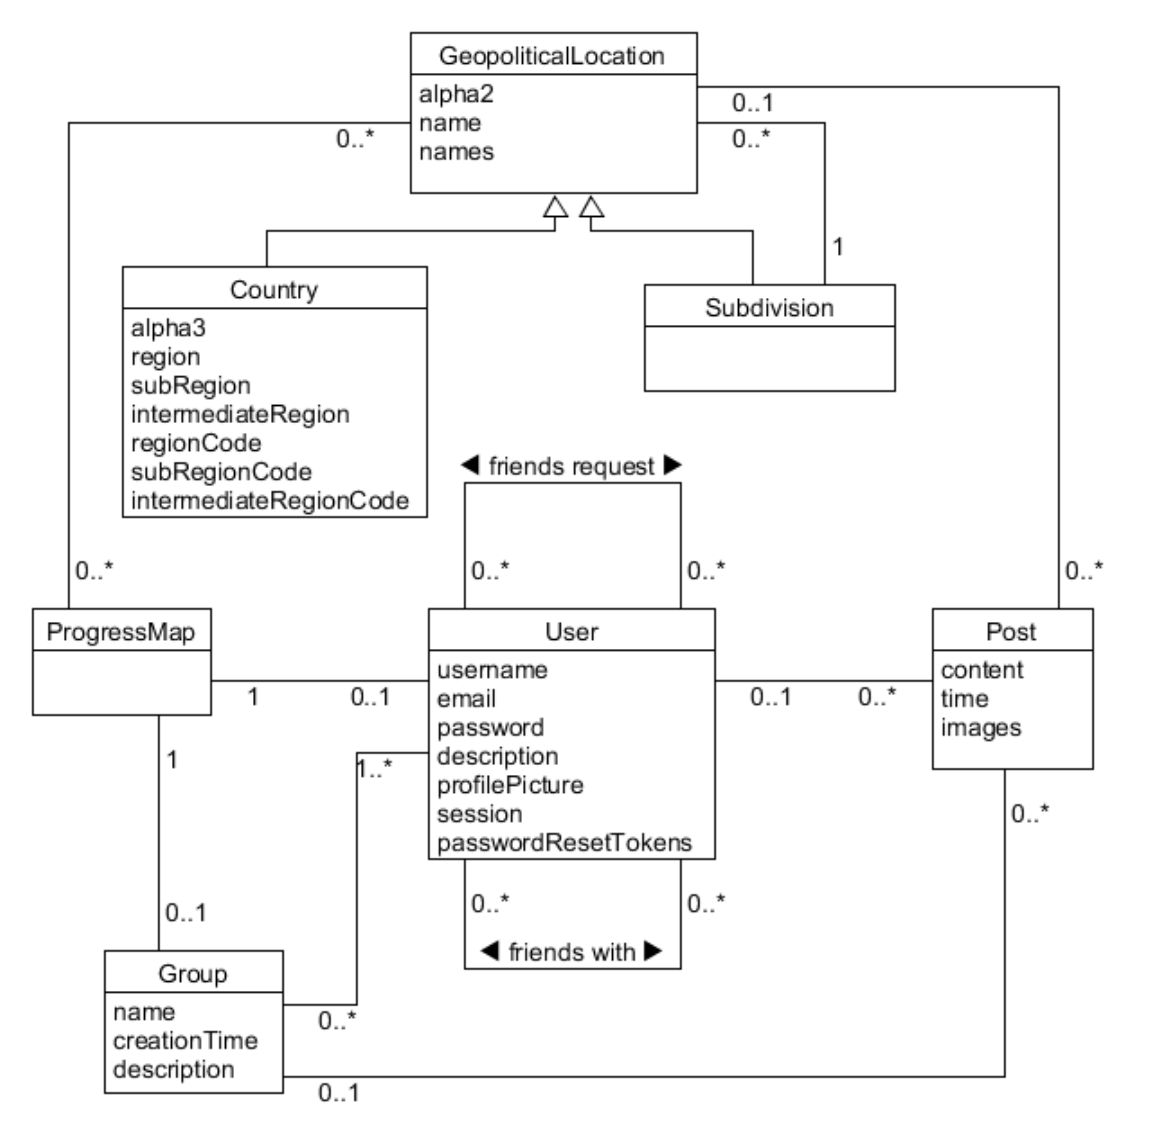
\includegraphics[width=\linewidth]{figures/Domain.png}
    \caption{Domain model}
    \label{fig:Domain}
\end{figure}

Domænemodellen viser forholdende mellem de forskellige model-klasser i systemet. Til at starte med var der kun User, ProgressMap, GeopoliticalLocation, Country og Subdivision, da fokus var på at brugeren skulle kunne bruge deres eget kort til at se hvor meget af verden de havde set. Senere blev der introduceret Post, friends og friends requests, samt Group, sådan at man nu kunne dele sin profil og kort med sine venner. 
Formålet var at det så skulle være muligt at deles om et ProgressMap i en gruppe, og deles om opslag - det er her samtidighedsproblemet i projektet kommer i fokus.
% Write about what choices we made with regards to concurrency.

\begin{figure}
    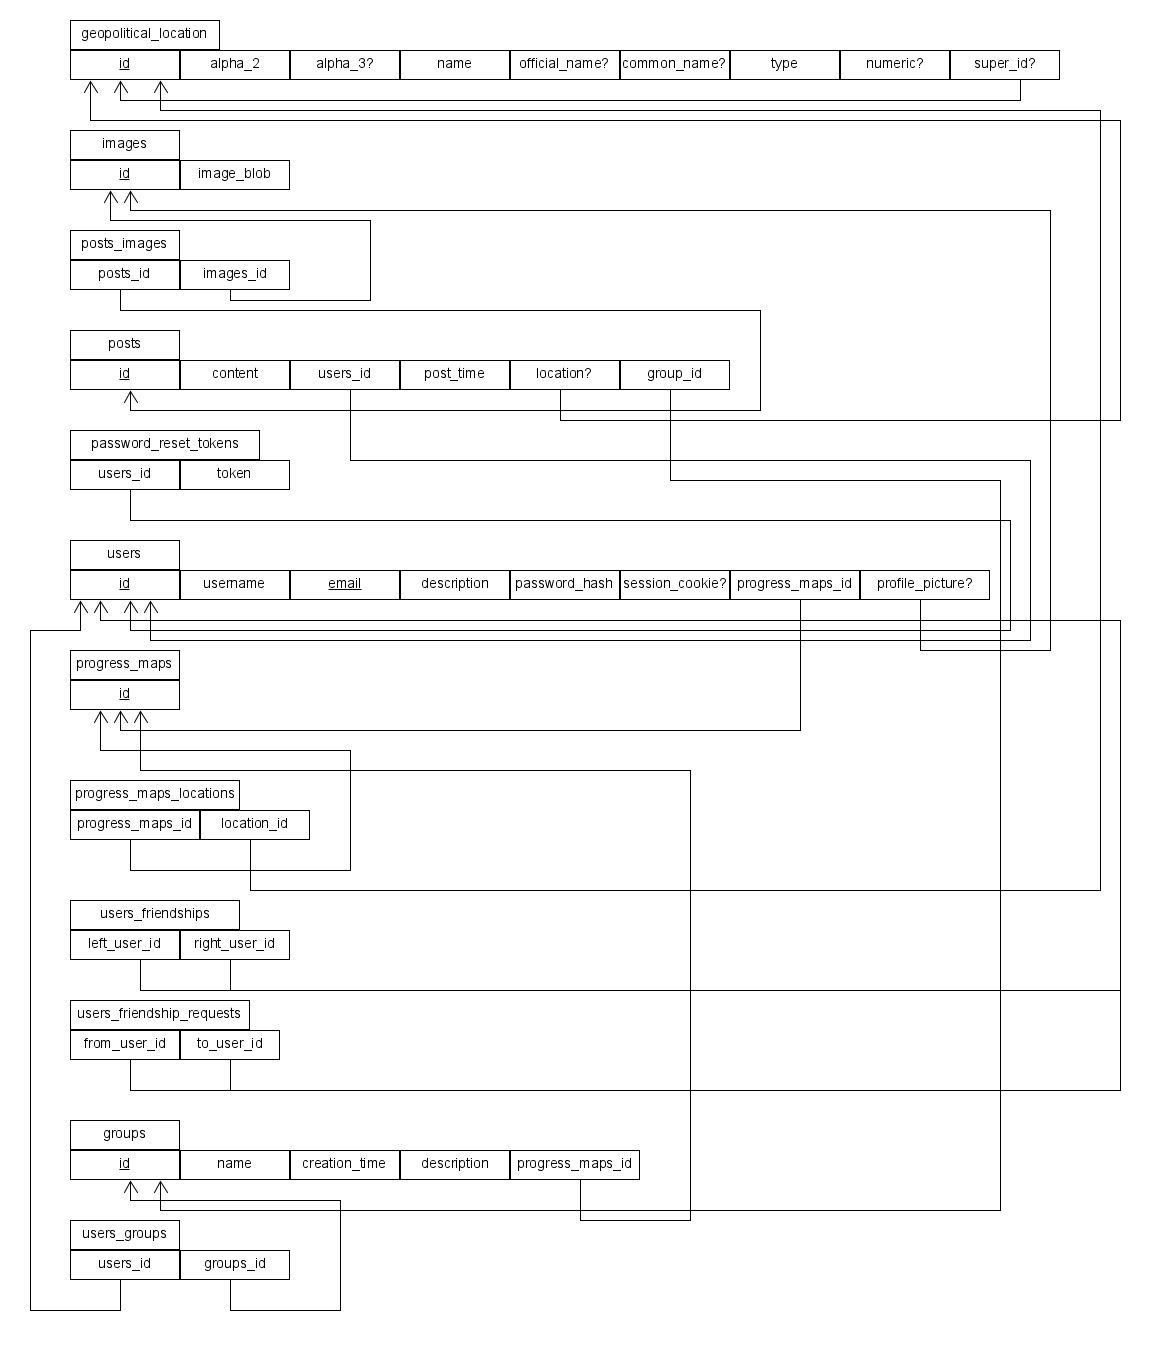
\includegraphics[width=\linewidth]{figures/RelationelmModel.png}
    \caption{Relationel Model}
    \label{fif:Rela}
\end{figure}

Den relationelle model afspejler domænemodellen, samt indeholder tabeller hvis formål er at håndtere forholdene mellem model-klasserne, herunder 1-1, 1-mange, og mange-mange forhold. Dette kan ses på tabeller som \texttt{progress\_maps\_locations}, \texttt{users\_friendships}, \texttt{users\_friendship\_requests}, \texttt{users\_groups} og \texttt{posts\_images}. Modellen opfylder ikke samtlige krav til BCNF\cite{bcnf}, og det kan ses to steder: \texttt{geopolitical\_location} indeholder \texttt{name} som ikke er atomisk. Dette skyldes at hvert land kan have flere officielle navne, uden at det påvirker samtlige andre data. Eksempelvis kan Storbrittanien også hedde United Kingdom og UK. Udover dette lagrer vi heller ikke hvert lands indelinger, da det ikke giver mening at lagre data som ikke bruges til noget. 

Ud fra systemets arkitektur, kan teamet fokusere på at udvikle softwaren med respekt til designet. For at skabe den bedst mulige kvaliet af software, har teamet fokuseret på at kvalitetssikre processen. I næste afsnit vil der blive introduceret FURPS+ og bestemte XP praktikker, som er benyttet til at kvalitetssikre produktet. 